\documentclass[12pt, letterpaper]{article}
\usepackage{graphicx} % Required for inserting images
\usepackage{hyperref}
\usepackage{listings}
\usepackage{amssymb}
\usepackage{amsmath}
\usepackage[english]{babel}
\usepackage{nicefrac, xfrac}
\usepackage{mathtools}
\usepackage[table,xcdraw]{xcolor}
\definecolor{light-gray}{gray}{0.95}
\definecolor{sap}{RGB}{130, 36, 51}
\definecolor{lg}{RGB}{102, 161, 95}
\definecolor{g}{RGB}{60, 50, 50}
\usepackage[paper=a4paper,left=20mm,right=20mm,bottom=25mm,top=25mm]{geometry}
\newcommand{\code}[1]{\colorbox{light-gray}{\texttt{#1}}}
\newcommand{\shelll}[1]{\colorbox{black}{\textcolor{white}{\texttt{#1}}}}
\newcommand{\shell}[1]{\colorbox{black}{\textcolor{white}{\texttt{casufrost@debian:$\sim$\$ #1}}}}
\newcommand{\codee}[1]{\colorbox{white}{\texttt{#1}}}
\newcommand{\acc}{\\\hphantom{}\\}
\newcommand{\dete}{{\rightarrow}}
\newcommand{\fdot}{{\(\bullet\) }}
\newcommand{\comm}[1]{\color{lg}\textit{\hphantom{spaz}// \text{#1}}\color{black}}
\newcommand{\textg}[1]{\color{g}{\textbf{#1}}\color{black}}
\newcommand{\boxedMath}[1]{\begin{tabular}{|c|}\hline \texttt{#1} \\ \hline\end{tabular} :}
\title{Reti di Elaboratori}
\author{Marco Casu}
\date{\vspace{-5ex}}
\begin{document}
\begin{center}
    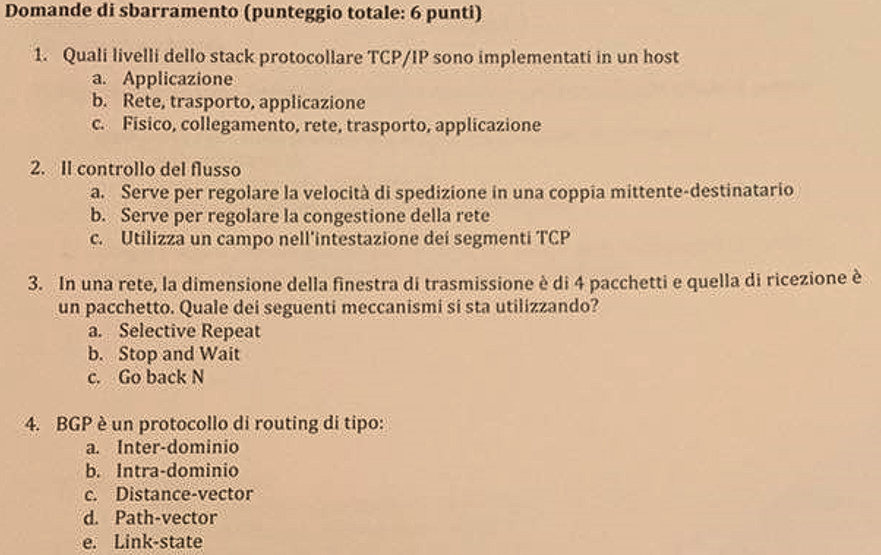
\includegraphics[width=0.8\textwidth ]{sbarramento.png}
\end{center}
\textbf{Soluzione} :
\begin{enumerate}
    \item (b) - Rete, trasporto, applicazione 
    \item (c) - Utilizza un campo nell'intestazione dei segmenti TCP 
    \item (c) - Go back N 
    \item \color{red}Domanda riguardante argomenti
    non ancora presentati 
    nel programma oggi 01/04/2024\color{black}
\end{enumerate}
\hphantom{text}\acc
\begin{center}
    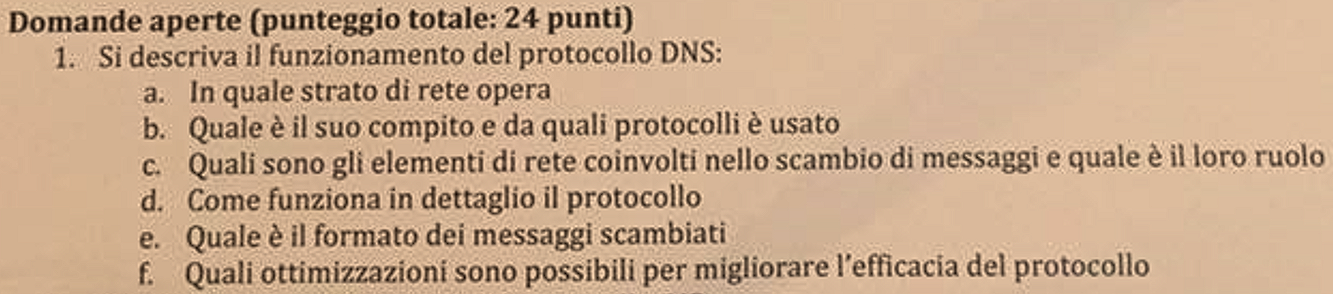
\includegraphics[width=0.8\textwidth ]{aperte1.png}
\end{center}
\textbf{(a)} - Il protocollo DNS opera nel livello di applicazione.\\ 
\textbf{(b)} - Il suo compito è quello di fornire la traduzione fra domini ed indirizzi 
IP, fornire degli alias per il nome canonico di un host, fornire un alias per il 
server mail associato, e distribuire il carico riguardante il processo di traduzione. I 
messaggi DNS sono incapsulati in UDP.\\
\textbf{(c)} - Gli elementi coinvolti sono, l'host che richiede la traduzione, il server DNS 
locale che si occupa di ricercare la traduzione, ed i server DNS che si occupano di fornire le traduzioni, 
o indicare altri server DNS che potrebbero esserne in possesso.\\
\textbf{(d)} - Esiste un database distribuito fra vari DNS server sparsi nel mondo, alcuni sono detti 
TDL e sono responsabili dei domini principali come \code{.net} o \code{.com}, in cima a tutti vi è il 
root server. I vari enti che vogliono registrare un dominio devono fornire una traduzione configurando il loro 
server DNS, un server DNS può conservare anche record di cui non è responsabile, ma essi non saranno considerati 
"autoritari". Il server di root fornisce indicazione sui server DNS TDL, e questi ultimi forniscono indicazioni sui loro 
sotto-domini e così via in maniera gerarchica. Se un host vuole richiedere il dominio \code{prime.amazon.it}, 
verrà interrogato il root server, esso fornirà le informazioni di \code{.it}, quest'ultimo le informazioni di 
\code{amazon.it}, e quest'ultimo ancora fornirà all'host la traduzione di \code{prime.amazon.it}.
\\\textbf{(e)} - Il formato dei messaggi è binario.\\ 
\textbf{(f)} - I server DNS locali possono mantenere una cache con i record del database in modo 
da fornire i record più rapidamente e non congestionare la rete.\acc 
\color{red}La domanda 2 sarà omessa in quanto riguardante argomenti non ancora presentati 
nel programma oggi 01/04/2024\color{black}\hphantom{text}\acc
\begin{center}
    
\includegraphics[width=0.8\textwidth ]{aperte3.png}
\end{center}
\textbf{(a)} - I numeri di sequenza dei segmenti rappresentano il numero del primo byte (rispetto al flusso totale 
di byte) presente all'interno del segmento in questione. Se un segmento contiene i byte dal 45 al 1400, avrà numero di 
segmento 45.\\
\textbf{(b)} - Quando si invia un segmento, per accertarsi del fatto che sia stato consegnato, il destinatario notifica 
il mittente con un messaggio detto ACK. All'invio di un segmento, partirà un timer, se entro la scadenza di quel timer non 
si sarà ricevuto un ACK, tale segmento sarà considerato perso, e verrà ritrasmesso in automatico. Ciò avviene anche 
al ricevimento di 3 ACK duplicati.\\ 
\textbf{(c)} - Il retrasmission time out al per il segmento $t$ è calcolato nel seguente modo:

$$ RTTestimated(t) = \text{RTT stimato per il segmento }t $$
$$ sampleRTT(t) = \text{RTT effettivo misurato per il segmento }t$$
$$ \alpha,\beta \in [0,1] \text{ pesi}$$
$$  RTTestimated(t+1)=RTTestimated(t)\cdot(1-\alpha) + sampleRTT(t)\cdot \alpha$$ 
$$ DevRTT(t+1) = (1-\beta) \cdot DevRTT(t)+\beta\cdot (|sampleRTT(t)-RTTestimated(t)|)$$
    $$RetrasmissionTimeOut(t) = RTTestimated(t)+4\cdot DevRTT(t) $$

\end{document}